\documentclass{../../sheet}
\renewcommand{\logopath}{../../logos/}

\title{PSE Vorkurs Tag 5}

\begin{document}
\maketitle
Heute Abend UNO!

\newpage
\aufgabe{Aufgabe 1: Maps}
Maps verbinden ein Schlüsselelement mit einem Wert. Diese können auch unterschiedliche Datentypen haben. Ein Telefonbuch könnte beispielsweise als Map dargestellt werden um Namen mit Telefeonnummern zu verbinden:
\begin{minted}[linenos=false]{java}
Map<String, Integer> telefonbuch = new HashMap<String, Integer>();
//erstes Parameter ist der Schlüssel, zweites ist der Wert
telefonbuch.put("Paul Griller", 1374927394);
\end{minted}

\begin{enumerate}
    \item Erstelle einen neue String-Variable mit dem folgenden Text:
    \begin{ausgabe}
        Grimmige Griller grillen glühend gern grobe Grillgemüse-Spieße.
    \end{ausgabe}
    \item Schreibe einen Algorithmus der in einem Dictionary speichert, wie oft jeder Buchstabe im String vorkommt. 

    Hinweis: Verwende die split("") Methode auf einen String in ein Zeichenarray umzuwanden. Mehr dazu findest du hier: \url{https://docs.oracle.com/javase/8/docs/api/java/lang/String.html#split-java.lang.String-}.

    \item Schreibe eine Funktion die ein Dictionary entgegennimmt und alle Schlüssel und die dazugehörigen Werte ausgibt.
    
    Lösung:
    \begin{ausgabe}
        b: 1, d: 1, e: 10, g: 9, h: 1, i: 6, l: 7, m: 3, n: 3, o: 1, p: 1, r: 7, s: 2, ß: 1, ü: 2
    \end{ausgabe}
\end{enumerate}

\newpage
\aufgabe{Aufgabe 2: Datenstrukturen selber machen}
Man kann sich in Java jederzeit selbst eine eigene Datenstruktur bauen, die dann auch an die eigenheiten der Problemstellung angepasst sein kann. Ihr habt ja sicher schon gemerkt, das Arrays etwas sperrig zu nutzen sind, da deren Größe komplett statisch ist. Unsere Liste soll aus einzelnen Knotenklassen bestehen, die dann untereinander verbunden werden.
\begin{enumerate}
    \item Erstelle eine Knotenklasse namens \texttt{Node}. Jede Knotenklasse soll einen Wert \texttt{value} vom Typ \texttt{int}, sowie einen Folgeknoten \texttt{nextNode} vom Typ \texttt{Node} als Attribute haben. Erstelle einen sinnvollen Konstruktor.\\\\
    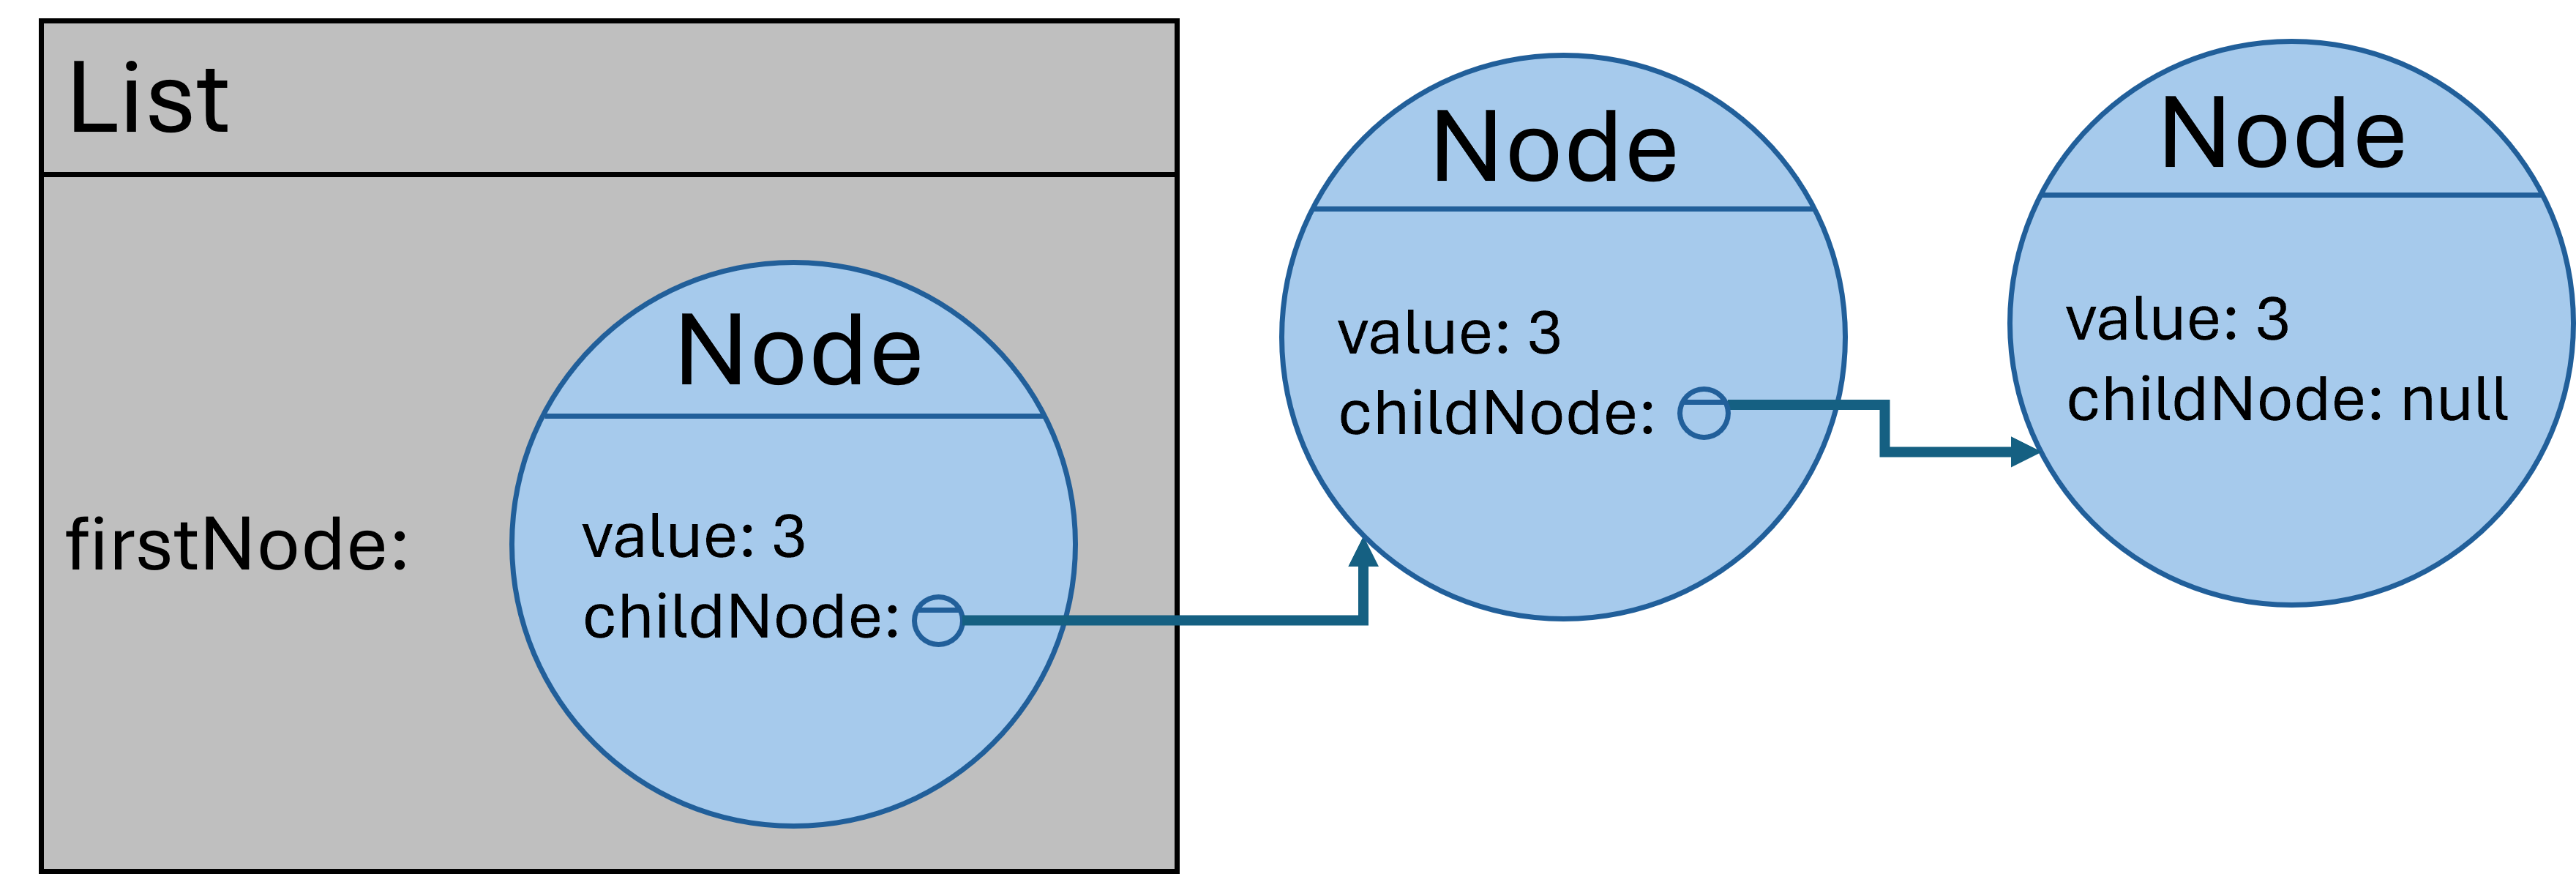
\includegraphics[width=\linewidth]{img/linkedlist.png}
    \item Erstelle jetzt die Listenklasse. Jede \texttt{List} hat einen Startknoten \texttt{startNode}. Programmiere wieder einen sinnvollen Konstruktor.
    \item Noch besteht jede dieser Listen nur aus einem einzelnen Startknoten. Füge um das zu ändern der \texttt{List} Klasse eine \texttt{add(Node newElement)} Funktion hinzu. Sie soll eine neue Node ans Ende der Liste anfügen. 
    \item Gib der \texttt{List} Klasse außerdem eine \texttt{remove(Node element)} Funktion. Achte darauf, dass dabei eventuelle Folgeelemente nicht ''Elternlos'' zurückgelassen werden. 
    \item Programmiere eine \texttt{printElements()} Funktion, die alle Elemente in der Liste anschaulich in der Konsole ausgibt.
    \item Schreibe eine Funktion, die die Summe der Elemente in der Liste berechnet. Schreibe dazu eine Funktion in der Klasse Node, die eine Summe entgegennimmt, ihren eigenen Wert hinzuaddiert und sich dann im nächsten Knoten selbst aufruft. Wenn die Methode auf den letzten Knoten in der Liste stößt, soll die berechnete Gesamtsumme auf der Konsole ausgegeben werden. Füge zuletzt der Klasse „List“ eine Funktion hinzu, die die Summenfunktion im ersten Knoten aufruft.
\end{enumerate}

Du hast gerade eine einfache LinkedList programmiert. LinkedLists sind sehr wichtig als Datenstruktur mit Variabler Größe und sie existieren auch in nativem Java: \url{https://docs.oracle.com/javase/8/docs/api/java/util/LinkedList.html}

\newpage
\aufgabe{HIGHPERFORMER-Aufgabe: Bäume}
Bäume sind auch eine wichtige Datenstruktur in Java. Bei einem Baum ist jeder Knoten mit Kindknoten verbunden, welche wiederum mit weiteren Kindknoten verbunden sind. So werden die Daten in einer Baumstruktur gespeichert:
\\
\begin{center}
    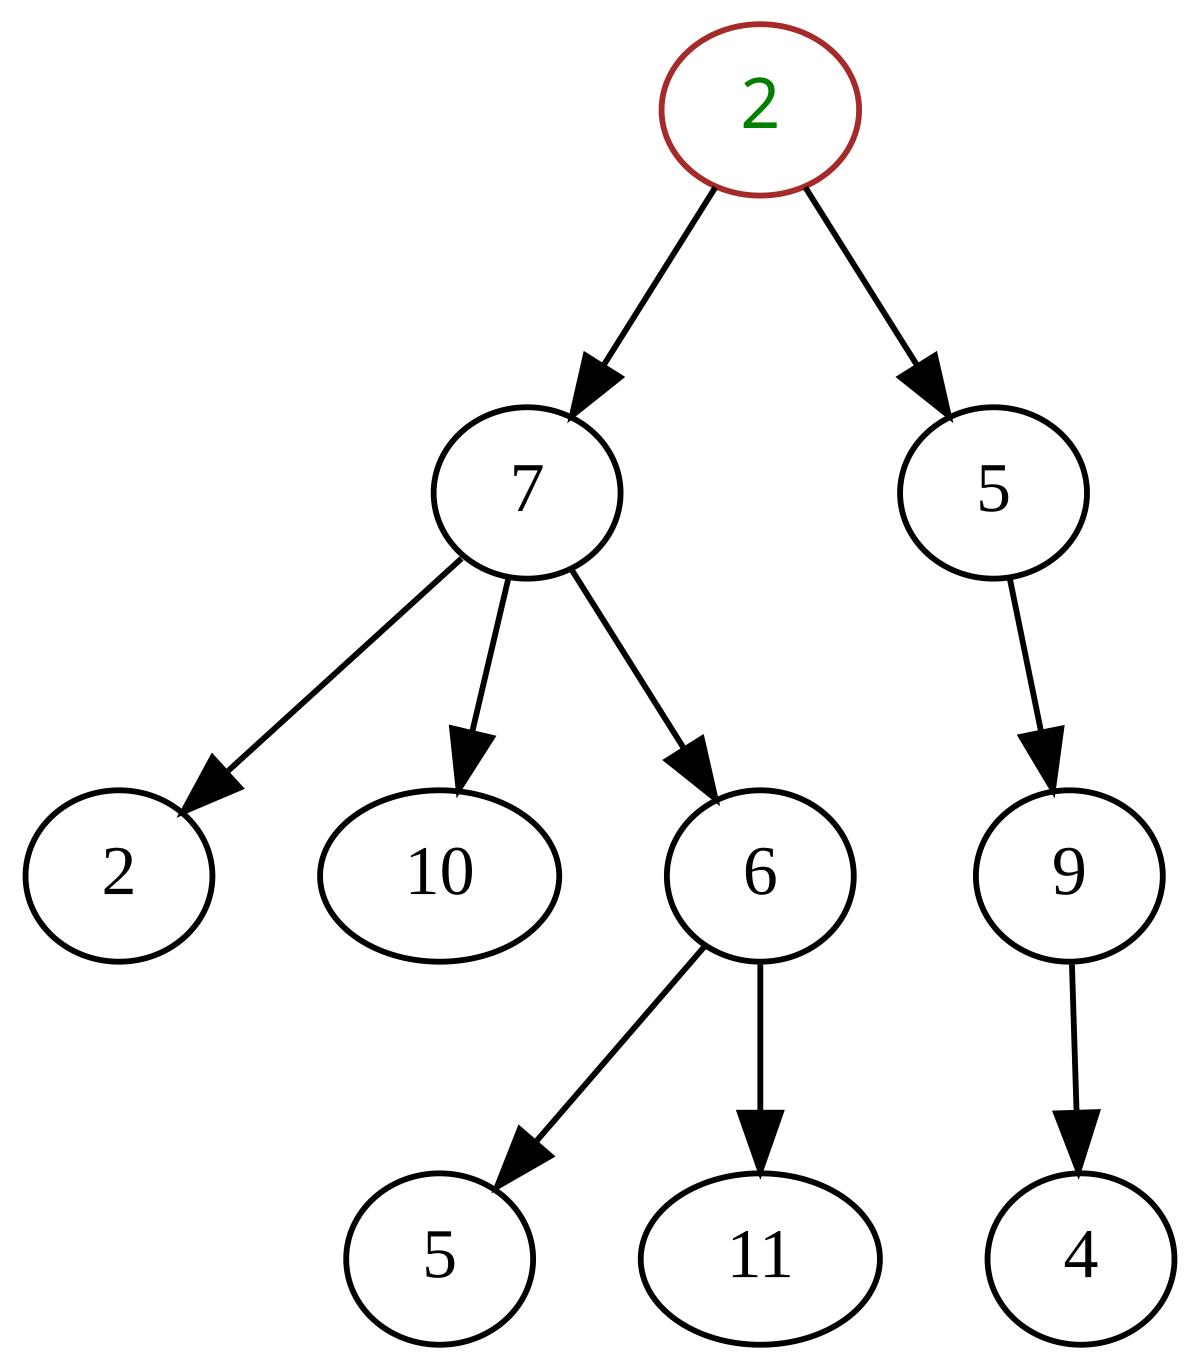
\includegraphics[width=0.5\linewidth]{img/baum.png}    
\end{center}

\begin{enumerate}
    \item Erstelle eine \texttt{Baum}-Klasse, die einen Wurzelknoten besitzt, sowie eine \texttt{Knoten}-Klasse, die einen \texttt{int}-Wert, sowie genau zwei Kindknoten (\texttt{linkesKind} und \texttt{rechtesKind}) speichert. Wenn ein Knoten bspw. kein rechtes Kind hat soll der Wert von \texttt{rechtesKind} gleich \texttt{null} sein. Da jeder Knoten maximal zwei Kinder ist der Baum ein sogenannter binärer Baum. 
    \item Programmiere eine Funktion in der \texttt{Baum}-Klasse, die eine neue Zahl in den Baum einfügt. Diese Funktion soll den Baum Knoten für Knoten durchgehen und bei jedem Knoten zufällig zum rechten oder linken Kind ''abbiegen''. Sobald auf ein \texttt{null} gestoßen wird, wird der einzufügende Wert dort mit einem neuen Knoten hinzugefügt. 
    \item Programmiere eine Funktion in der \texttt{Baum}-Klasse, die den Baum anschaulich ausgibt.
    \item Programmiere zwei Funktionen, die den Baum eindeutig in eine LinkedList umwandelt und eine die dasselbe umgekehrt macht. Überlege dir hierfür eine Möglichkeit wie man die Struktur eines Baums in der Liste abbilden kann. 
    Hinweis: Du kannst deine Funktionen Testen indem du einen Baum zu einer LinkedList umwandeln lässt und dann mit der anderen Funktion zurück zu einem Baum umwandelst und dann prüfst ob die Struktur erhalten geblieben ist. 
\end{enumerate}

\end{document}